\begin{figure}[H]
    \centering
    \definecolor{densityblue}{RGB}{35,105,180}
    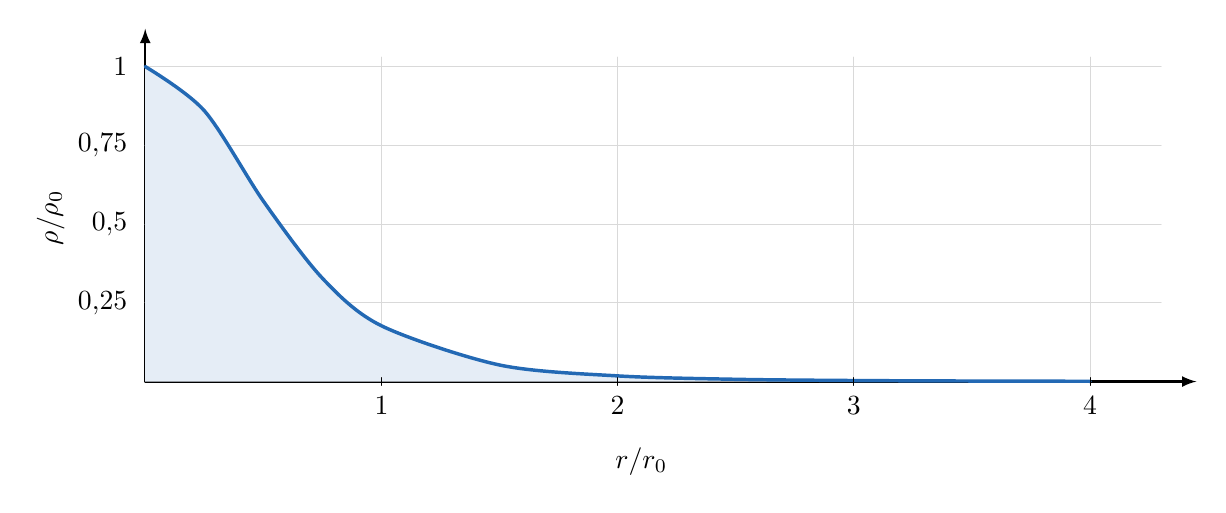
\begin{tikzpicture}[x=3.0cm,y=4.0cm,line cap=round,line join=round]
        \draw[-latex,line width=0.8pt] (0,0) -- (4.45,0);
        \draw[-latex,line width=0.8pt] (0,0) -- (0,1.12);
        \foreach \x in {1,2,3,4} {
            \draw[black!15] (\x,0) -- (\x,1.03);
        }
        \foreach \y in {0.25,0.5,0.75,1.0} {
            \draw[black!15] (0,\y) -- (4.30,\y);
        }

        \fill[densityblue!12]
            (0,0) --
            plot[smooth] coordinates {
                (0,1) (0.25,0.86) (0.5,0.573) (0.75,0.328)
                (1,0.177) (1.5,0.0525) (2,0.0179)
                (2.5,0.0071) (3,0.0032) (3.5,0.0016) (4,0.00084)
            } -- (4,0) -- cycle;

        \draw[densityblue,line width=1.25pt,smooth]
            plot coordinates {
                (0,1) (0.25,0.86) (0.5,0.573) (0.75,0.328)
                (1,0.177) (1.5,0.0525) (2,0.0179)
                (2.5,0.0071) (3,0.0032) (3.5,0.0016) (4,0.00084)
            };

        \node[anchor=north] at (2.10,-0.18) {$r/r_0$};
        \node[rotate=90] at (-0.40,0.52) {$\rho/\rho_0$};

        \foreach \x in {1,2,3,4} {
            \draw (\x,0.012) -- (\x,-0.012);
            \node[anchor=north] at (\x,-0.018) {$\x$};
        }
        \node[anchor=east] at (-0.035,0.25) {$0{,}25$};
        \node[anchor=east] at (-0.035,0.5) {$0{,}5$};
        \node[anchor=east] at (-0.035,0.75) {$0{,}75$};
        \node[anchor=east] at (-0.035,1) {$1$};
    \end{tikzpicture}
    \caption{Distribución normalizada de densidad obtenida en la parte (a) del problema 6.}
\end{figure}
